\section{有限差分}
\label{sec:zo-finite-differences}

只凭几个函数值，怎样得到梯度的近似？思路来自一元微积分：导数是割线斜率的极限，步子小一点，割线斜率就接近导数。

\paragraph{从一元差商开始}
设$\varphi(s)$是一元函数，$h>0$是\term{扰动尺度}（perturbation scale）。两种常用的\term{差商}（difference quotient）是\term{前向差分}（forward difference）和\term{中心差分}（central difference）：
\begin{equation}
 \frac{\varphi(s+h)-\varphi(s)}{h},\qquad
 \frac{\varphi(s+h)-\varphi(s-h)}{2h}.
 \label{eq:zo-quotients-1d}
\end{equation}
图~\ref{fig:zo-secants}用$\varphi(s)=s^2/2+s^3/6$，$s_0=1$，$h=0.8$画出两条割线和切线。切线斜率是$\varphi'(1)=1.5$。

由$\varphi(1)=2/3$、$\varphi(1.8)=2.592$和$\varphi(0.2)\approx0.0213$，两种差商是
\[
 \frac{2.592-0.6667}{0.8}\approx2.407,\qquad
 \frac{2.592-0.0213}{1.6}\approx1.607.
\]
前向差商偏离$0.907$，中心差商只偏离$0.107$。原因是Taylor展开的二次项：前向割线把弯曲全部算进了斜率，中心割线的两侧弯曲互相抵消。

\begin{BookInlineFigure}
  \centering
  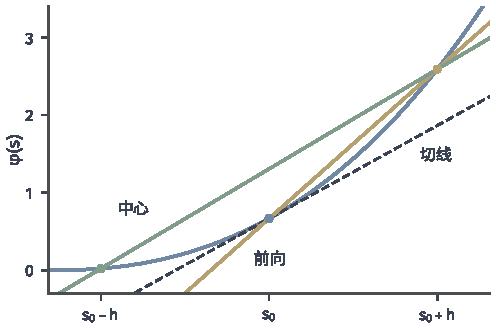
\includegraphics[width=84mm]{figures/05-optimization/05-stochastic-optimization/matplotlib/zo-secants/figure.pdf}
  \caption{$\varphi(s)=s^2/2+s^3/6$（蓝线）在$s_0=1$处的两种差商，$h=0.8$。虚线是切线，斜率$1.5$；黄线是前向割线，斜率约$2.407$；绿线是中心割线，斜率约$1.607$，方向最接近切线。}
  \label{fig:zo-secants}
\end{BookInlineFigure}

\paragraph{多元函数：沿一个方向看}
差商搬到多元函数上，只要限制在一条直线上。令$\varphi(s)=f(\bm{x}+s\bm{u})$，由链式法则$\varphi'(0)=\langle\nabla f(\bm{x}),\bm{u}\rangle$，这是方向导数。于是沿$\bm{u}$的中心差商近似$\langle\nabla f(\bm{x}),\bm{u}\rangle$。一次差商只告诉我们梯度在一个方向上的投影，要拼出整个梯度，需要多个方向，或者后面将看到的随机化。

下面的引理量化差商的\term{截断误差}（truncation error），它只涉及函数本身，不涉及噪声。第~\ref{chap:smooth-foundations}章的下降引理给出：$\nabla f$是$L$-Lipschitz时，对任意$\bm{x},\bm{v}$，
\[
 \bigl\lvert f(\bm{x}+\bm{v})-f(\bm{x})-\langle\nabla f(\bm{x}),\bm{v}\rangle\bigr\rvert
 \leq\frac{L}{2}\lVert\bm{v}\rVert_2^2.
\]

\begin{lemma}[差商的余项]
\label{lem:zo-remainder}
设$\nabla f$是$L$-Lipschitz的。对任意$\bm{x},\bm{v}$，
\begin{equation}
 \bigl\lvert f(\bm{x}+\bm{v})-f(\bm{x}-\bm{v})-2\langle\nabla f(\bm{x}),\bm{v}\rangle\bigr\rvert
 \leq L\lVert\bm{v}\rVert_2^2.
 \label{eq:zo-central-L}
\end{equation}
若$f$还二阶连续可微，且$\nabla^2f$按谱范数是$M$-Lipschitz的，则
\begin{equation}
 \bigl\lvert f(\bm{x}+\bm{v})-f(\bm{x}-\bm{v})-2\langle\nabla f(\bm{x}),\bm{v}\rangle\bigr\rvert
 \leq\frac{M}{3}\lVert\bm{v}\rVert_2^3.
 \label{eq:zo-central-M}
\end{equation}
\end{lemma}

\begin{proof}
把上面的不等式分别用于$\bm{v}$和$-\bm{v}$，两式相减，由三角不等式得式~\eqref{eq:zo-central-L}。

对第二个结论，记$\bm{H}=\nabla^2f(\bm{x})$。积分形式的Taylor公式给出
\[
 \begin{aligned}
 &f(\bm{x}+\bm{v})-f(\bm{x})-\langle\nabla f(\bm{x}),\bm{v}\rangle-\frac12\bm{v}^\top\bm{H}\bm{v}\\
 &\quad=\int_0^1(1-s)\,\bm{v}^\top\bigl(\nabla^2f(\bm{x}+s\bm{v})-\bm{H}\bigr)\bm{v}\,\mathrm{d}s.
 \end{aligned}
\]
右端的绝对值不超过
\[
 \int_0^1(1-s)\,Ms\,\lVert\bm{v}\rVert_2^3\,\mathrm{d}s=\frac{M}{6}\lVert\bm{v}\rVert_2^3.
\]
对$\bm{v}$和$-\bm{v}$各写一次再相减，二次项$\tfrac12\bm{v}^\top\bm{H}\bm{v}$恰好相消，余项相加得$\tfrac{M}{3}\lVert\bm{v}\rVert_2^3$。
\end{proof}

\paragraph{三笔账}
每种差分都要记三笔账。第一笔是截断误差，随$h$变小而变小。第二笔是读数噪声造成的误差：独立噪声方差$\sigma^2$时，前向差商的噪声是$(\zeta_1-\zeta_0)/h$，中心差商的噪声是$(\zeta_+-\zeta_-)/(2h)$，方差分别为
\begin{equation}
 \frac{2\sigma^2}{h^2},\qquad\frac{\sigma^2}{2h^2},
 \label{eq:zo-quotient-noise}
\end{equation}
都随$h$变小而变大。第三笔是查询次数。这三笔账彼此独立，下面逐个方法记录，第~\ref{sec:zo-tradeoff}节再做取舍。

\subsection{坐标差分}
\label{sec:zo-coordinate}

最直接的做法是沿$n$个坐标方向逐个差分，用$n$个方向导数拼成梯度。记$\bm{e}_i$为第$i$个标准基向量，两种\term{坐标差分}（coordinate difference）的第$i$个分量是
\begin{equation}
 \hat{g}^{\mathrm{F}}_i=\frac{f(\bm{x}+h\bm{e}_i)-f(\bm{x})}{h},\qquad
 \hat{g}^{\mathrm{C}}_i=\frac{f(\bm{x}+h\bm{e}_i)-f(\bm{x}-h\bm{e}_i)}{2h}.
 \label{eq:zo-coordinate}
\end{equation}

\paragraph{查询次数}
前向差分的$n$个分量可以共用中心读数$f(\bm{x})$，所以一共$n+1$次查询。中心差分每个坐标读两点，共$2n$次，中心点本身不读。图~\ref{fig:zo-stencils}(a)(b)画出了这两种查询模式。

\begin{BookInlineFigure}
  \centering
  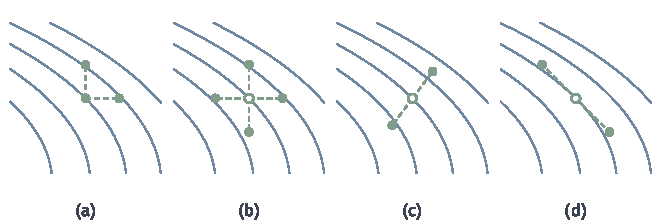
\includegraphics[width=112mm]{figures/05-optimization/05-stochastic-optimization/matplotlib/zo-stencils/figure.pdf}
  \caption{贯穿例在$(9,1)$附近的查询点，蓝线是等高线，为便于观察取$h=0.4$。实心点要读函数值，空心点是当前点、不读。(a)前向坐标差分，$3$次。(b)中心坐标差分，$4$次。(c)沿$\bm{u}=(0.6,0.8)$的随机方向差分，$2$次。(d)第~\ref{sec:zo-spsa}节的同时扰动，$\bm{\Delta}=(1,-1)$，$2$次，位移长度是$h\sqrt{2}$。}
  \label{fig:zo-stencils}
\end{BookInlineFigure}

\paragraph{手算比较}
在贯穿例的起点取$h=0.1$。为算前向差商，读三个函数值：
\[
 f(9,1)=45,\qquad f(9.1,1)=45.905,\qquad f(9,1.1)=45.945.
\]
代入式~\eqref{eq:zo-coordinate}，前向差分给出
\[
 \hat{\bm{g}}^{\mathrm{F}}=(9.05,\ 9.45).
\]
真实梯度是$(9,9)$，误差$(0.05,\,0.45)$，恰好等于$\tfrac{h}{2}H_{ii}$：沿$x_2$方向弯曲是$x_1$方向的$9$倍，误差也是$9$倍。

再读$f(8.9,1)=44.105$和$f(9,0.9)=44.145$，中心差分给出
\[
 \hat{\bm{g}}^{\mathrm{C}}=\Bigl(\frac{45.905-44.105}{0.2},\ \frac{45.945-44.145}{0.2}\Bigr)=(9,\ 9).
\]
对二次函数，中心差分没有截断误差，因为三阶以上的导数都是零。多付一次查询，换来了精确值。

\paragraph{截断误差的一般结论}
上面的现象对一般函数也成立，只是阶数要由相应的导数条件来保证。

\begin{theorem}[坐标差分的截断误差]
\label{thm:zo-coordinate}
设读数精确。若$\nabla f$是$L$-Lipschitz的，则
\begin{equation}
 \lVert\hat{\bm{g}}^{\mathrm{F}}-\nabla f(\bm{x})\rVert_2\leq\frac{\sqrt{n}\,Lh}{2}.
 \label{eq:zo-coordinate-forward}
\end{equation}
若$f$还二阶连续可微且$\nabla^2f$是$M$-Lipschitz的，则
\begin{equation}
 \lVert\hat{\bm{g}}^{\mathrm{C}}-\nabla f(\bm{x})\rVert_2\leq\frac{\sqrt{n}\,Mh^2}{6}.
 \label{eq:zo-coordinate-central}
\end{equation}
\end{theorem}

\begin{proof}
对前向差分，把下降引理用于$\bm{v}=h\bm{e}_i$，再除以$h$，得
\[
 \lvert\hat{g}^{\mathrm{F}}_i-\partial_if(\bm{x})\rvert\leq\frac{Lh}{2}.
\]

对中心差分，把式~\eqref{eq:zo-central-M}用于$\bm{v}=h\bm{e}_i$，再除以$2h$，得
\[
 \lvert\hat{g}^{\mathrm{C}}_i-\partial_if(\bm{x})\rvert\leq\frac{Mh^2}{6}.
\]
$n$个分量各不超过同一个上界，向量的欧氏范数不超过该上界乘以$\sqrt{n}$。
\end{proof}

定理的条件各有作用。前向差分只用到梯度的Lipschitz性，误差是一阶的。中心差分要快一阶，需要三阶信息受控，也就是Hessian的Lipschitz性；只有$L$时，由式~\eqref{eq:zo-central-L}只能得到每个分量$Lh/2$，与前向差分同阶。

图~\ref{fig:zo-trunc-log}在$\varphi(s)=s^2/2+s^3/6$上验证这两个阶数。双对数坐标下，前向误差的斜率是$1$，中心误差的斜率是$2$，$h$每缩小$10$倍，中心差分的误差缩小$100$倍。

\begin{BookInlineFigure}
  \centering
  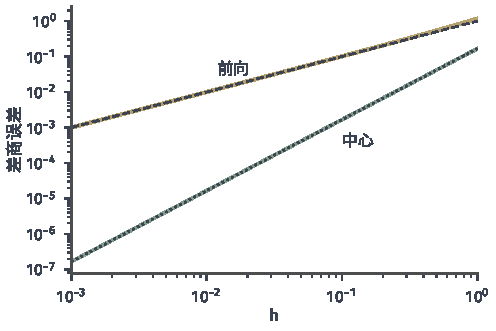
\includegraphics[width=84mm]{figures/05-optimization/05-stochastic-optimization/matplotlib/zo-trunc-log/figure.pdf}
  \caption{精确读数下差商误差随$h$的变化，$\varphi(s)=s^2/2+s^3/6$，$s_0=1$，真实导数$1.5$。黄线为前向差分，绿线为中心差分；虚线是$h$，点线是$h^2/6$，分别对应理论的斜率$1$和$2$。}
  \label{fig:zo-trunc-log}
\end{BookInlineFigure}

\subsection{随机方向差分}
\label{sec:zo-random-direction}

坐标差分每算一次梯度要$n$轮查询，维数大时一步也走不起。一个自然的想法是：每轮只沿一个方向差分，方向随机抽，多轮平均下来也许能覆盖各个方向。

\paragraph{从方向导数恢复向量}
一次差商是一个标量，要把它变成向量，乘上方向本身。设$\bm{u}$在单位球面$\bm{S}$（$\mathbb{R}^n$中全体长度为$1$的向量）上均匀分布。记$\bm{g}=\nabla f(\bm{x})$，考察$\langle\bm{g},\bm{u}\rangle\bm{u}$的均值。由对称性，$\mathbb{E}[u_iu_j]=0$（$i\neq j$），且$n$个$\mathbb{E}[u_i^2]$相等，和为$1$，所以
\[
 \mathbb{E}[\bm{u}\bm{u}^\top]=\frac{1}{n}\bm{I}.
\]
于是
\[
 \mathbb{E}\bigl[\langle\bm{g},\bm{u}\rangle\bm{u}\bigr]=\mathbb{E}[\bm{u}\bm{u}^\top]\bm{g}=\frac{1}{n}\bm{g}.
\]
乘以$n$就得到$\bm{g}$的无偏量。把方向导数换成中心差商，定义\term{随机方向差分}（random-direction difference）：
\begin{equation}
 D_h(\bm{u})=\frac{f(\bm{x}+h\bm{u})-f(\bm{x}-h\bm{u})}{2h},\qquad
 \hat{\bm{g}}=n\,D_h(\bm{u})\,\bm{u}.
 \label{eq:zo-random-direction}
\end{equation}
一般地，若方向分布满足$\mathbb{E}[\bm{u}\bm{u}^\top]=c\,\bm{I}$，归一化因子就是$1/c$。因子$n$来自单位球面的二阶矩，不是万能常数。

\paragraph{一条方向只有一条方向的信息}
在起点，贯穿例是二次函数，中心差商精确等于方向导数，$\hat{\bm{g}}=2\langle\bm{g},\bm{u}\rangle\bm{u}$。取几个方向，结果如下：
\[
 \bm{u}=(1,0):\ \hat{\bm{g}}=(18,0),\qquad
 \bm{u}=(0,1):\ \hat{\bm{g}}=(0,18).
\]
第三、第四个方向是$(1,1)/\sqrt{2}$和$(1,-1)/\sqrt{2}$，得到
\[
 \hat{\bm{g}}=(18,18),\qquad\hat{\bm{g}}=(0,0).
\]
四个估计的平均是$(9,9)$，但没有一个单独接近$(9,9)$。方向$(1,-1)/\sqrt{2}$与梯度垂直，一条差商得到零，什么也看不出来。

图~\ref{fig:zo-circle}(a)说明所有估计的分布：$n=2$时，$2\langle\bm{g},\bm{u}\rangle\bm{u}$走遍一个以$\bm{g}$为圆心、过原点的圆。圆心就是均值，半径就是误差的大小。单个估计总是偏离$\lVert\bm{g}\rVert_2$，只有平均才接近$\bm{g}$。

\begin{BookInlineFigure}
  \centering
  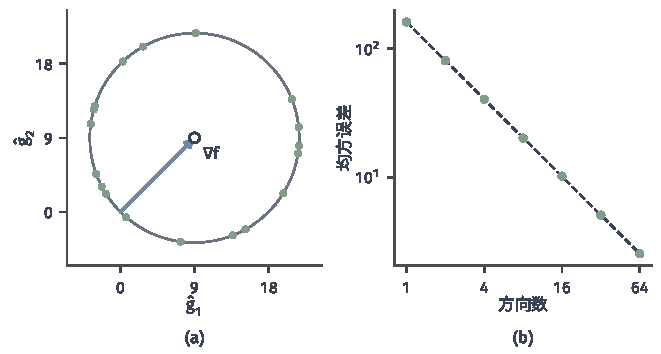
\includegraphics[width=112mm]{figures/05-optimization/05-stochastic-optimization/matplotlib/zo-circle/figure.pdf}
  \caption{贯穿例起点处$\bm{g}=(9,9)$的随机方向估计。(a)绿点是$18$个随机方向给出的$2\langle\bm{g},\bm{u}\rangle\bm{u}$，全部落在以$\bm{g}$（空心圆）为圆心、半径$\lVert\bm{g}\rVert_2$的灰圆上，蓝色箭头是真实梯度。(b)$m$个独立方向平均后的均方误差，绿点是Monte Carlo结果，虚线是$162/m$。}
  \label{fig:zo-circle}
\end{BookInlineFigure}

\paragraph{偏差与二阶矩}
下面的定理把偏差和波动分开。

\begin{theorem}[随机方向差分]
\label{thm:zo-random-direction}
设读数精确，$\bm{u}$在$\bm{S}$上均匀分布，$\hat{\bm{g}}$由式~\eqref{eq:zo-random-direction}定义。若$f$是二次函数，则
\begin{equation}
 \mathbb{E}[\hat{\bm{g}}]=\bm{g},\qquad
 \mathbb{E}\lVert\hat{\bm{g}}-\bm{g}\rVert_2^2=(n-1)\lVert\bm{g}\rVert_2^2.
 \label{eq:zo-direction-quadratic}
\end{equation}
若$f$二阶连续可微且$\nabla^2f$是$M$-Lipschitz的，则偏差满足
\begin{equation}
 \bigl\lVert\mathbb{E}[\hat{\bm{g}}]-\bm{g}\bigr\rVert_2\leq\frac{nMh^2}{6}.
 \label{eq:zo-direction-bias}
\end{equation}
\end{theorem}

\begin{proof}
二次函数的中心差商没有余项，$\hat{\bm{g}}=n\langle\bm{g},\bm{u}\rangle\bm{u}$，由$\mathbb{E}[\bm{u}\bm{u}^\top]=\bm{I}/n$得$\mathbb{E}[\hat{\bm{g}}]=\bm{g}$。

二阶矩用$\lVert\bm{u}\rVert_2=1$计算：
\[
 \mathbb{E}\lVert\hat{\bm{g}}\rVert_2^2=n^2\mathbb{E}\langle\bm{g},\bm{u}\rangle^2=n^2\cdot\frac{\lVert\bm{g}\rVert_2^2}{n}=n\lVert\bm{g}\rVert_2^2.
\]
减去均值的平方$\lVert\bm{g}\rVert_2^2$，得到方差。

一般情形写$D_h(\bm{u})=\langle\bm{g},\bm{u}\rangle+r$。把式~\eqref{eq:zo-central-M}用于$\bm{v}=h\bm{u}$并除以$2h$，得$\lvert r\rvert\leq Mh^2/6$。于是
\[
 \bigl\lVert\mathbb{E}[\hat{\bm{g}}]-\bm{g}\bigr\rVert_2=n\bigl\lVert\mathbb{E}[r\bm{u}]\bigr\rVert_2\leq n\,\mathbb{E}\lvert r\rvert\leq\frac{nMh^2}{6}.
\]
\end{proof}

式~\eqref{eq:zo-direction-quadratic}的$n-1$就是维数的代价：一条方向只探测了$n$维中的一维，其余$n-1$维的信息要靠多轮平均。图~\ref{fig:zo-circle}(b)验证了$m$个独立方向平均后，均方误差按$(n-1)\lVert\bm{g}\rVert_2^2/m$下降。

\paragraph{有限扰动下一般有偏}
二次函数上的无偏是特例。一旦有三阶项，中心差商不再等于方向导数，由它乘$\bm{u}$形成的向量，均值一般不等于原梯度。取$n=2$，$f(\bm{x})=x_1^3$，在$x_1=0$处真实梯度为零。差商和估计为
\[
 D_h(\bm{u})=h^2u_1^3,\qquad\hat{\bm{g}}=2h^2u_1^3\,\bm{u}.
\]
记$\bm{u}=(\cos\theta,\sin\theta)$。由$\mathbb{E}[\cos^4\theta]=\tfrac38$和$\mathbb{E}[\cos^3\theta\sin\theta]=0$，
\[
 \mathbb{E}[\hat{\bm{g}}]=\bigl(\tfrac34h^2,\ 0\bigr)\neq\bm{0}.
\]
这里$M=6$，定理的界是$2h^2$，实际偏差$\tfrac34h^2$在界内。偏差确实存在，而且随$h$平方缩小。

\subsection{同时扰动随机逼近}
\label{sec:zo-spsa}

随机方向差分要从球面上抽方向，并且需要因子$n$。Spall提出的\term{同时扰动随机逼近}（simultaneous perturbation stochastic approximation，SPSA）用更简单的方式达到类似的效果：让所有坐标同时动一下，每个坐标只取正负两个方向。

\paragraph{主要思想}
抽取向量$\bm{\Delta}\in\{-1,+1\}^n$，各分量独立，等可能取$\pm1$。查询两点$\bm{x}\pm h\bm{\Delta}$，算一个函数差，再把同一个差除以各分量的扰动：
\begin{equation}
 D=\frac{y_+-y_-}{2h},\qquad \hat{g}_i=\frac{D}{\Delta_i},\quad i=1,\ldots,n.
 \label{eq:zo-spsa}
\end{equation}
只读了两次，却得到了$n$个分量。为什么这样能行？若$f$是二次函数，$D=\langle\bm{g},\bm{\Delta}\rangle$，于是
\[
 \hat{g}_i=g_i+\sum_{j\neq i}g_j\frac{\Delta_j}{\Delta_i}.
\]
第一项是想要的。后面每一项都是其他坐标的“串扰”。因为$\Delta_j$与$\Delta_i$独立，且$\mathbb{E}[\Delta_j]=0$，串扰的均值是零，平均之后消失。

除法要求$\mathbb{E}[1/\lvert\Delta_i\rvert]$有限，这解释了分布的选择。正态或区间上的均匀扰动在$0$附近有正的密度，$1/\lvert\Delta_i\rvert$的期望发散，不能用于这个公式。$\pm1$时$1/\Delta_i=\Delta_i$，估计也可以写成$\hat{\bm{g}}=D\,\bm{\Delta}$。

\paragraph{手算四种情形}
贯穿例起点，$h=0.1$，$n=2$，$\bm{\Delta}$有四种等可能取值。取$\bm{\Delta}=(1,1)$，读数和差商是
\[
 y_+=f(9.1,1.1)=46.85,\qquad y_-=f(8.9,0.9)=43.25,\qquad D=18.
\]
取$\bm{\Delta}=(1,-1)$，两次读数相等，差商为零：
\[
 y_+=f(9.1,0.9)=45.05,\qquad y_-=f(8.9,1.1)=45.05,\qquad D=0.
\]
$-\bm{\Delta}$与$\bm{\Delta}$的结果相同。四种情形的估计分别是$(18,18)$、$(0,0)$、$(0,0)$、$(18,18)$，平均恰为$(9,9)$，如图~\ref{fig:zo-spsa}(b)。

\begin{BookInlineFigure}
  \centering
  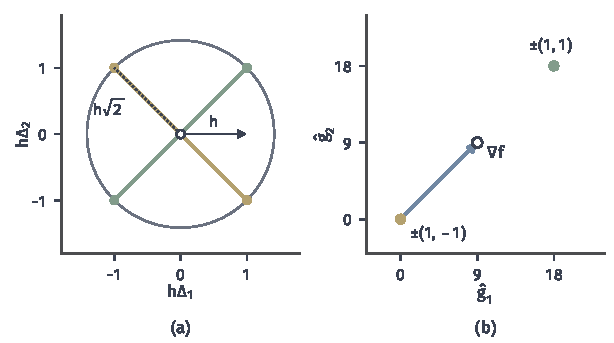
\includegraphics[width=104mm]{figures/05-optimization/05-stochastic-optimization/matplotlib/zo-spsa/figure.pdf}
  \caption{$n=2$时的同时扰动。(a)四个扰动$h\bm{\Delta}$（$h=1$）位于正方形顶点，一对相反的点共用一次差分，绿、黄各一对；每个坐标只动$h$，位移长度却是$h\sqrt{2}$，四点都在半径$h\sqrt{2}$的圆上。(b)贯穿例起点的估计，绿点是$\bm{\Delta}=\pm(1,1)$的结果，黄点是$\bm{\Delta}=\pm(1,-1)$的结果，它们的平均是真实梯度（空心圆）。}
  \label{fig:zo-spsa}
\end{BookInlineFigure}

\paragraph{偏差与噪声}
SPSA在原梯度上的偏差由差商余项决定，与随机方向差分的结论形式一样，只是这里的位移长度不再是$h$。

\begin{theorem}[SPSA的偏差]
\label{thm:zo-spsa}
设$f$二阶连续可微，$\nabla^2f$是$M$-Lipschitz的，$\bm{\Delta}$的分量独立且等可能取$\pm1$，读数为$y_\pm=f(\bm{x}\pm h\bm{\Delta})+\zeta_\pm$，且给定$\bm{x},\bm{\Delta}$时$\zeta_+-\zeta_-$的条件均值为零。则对$\hat{\bm{g}}$的每个分量，
\begin{equation}
 \bigl\lvert\mathbb{E}[\hat{g}_i\mid\bm{x}]-\partial_if(\bm{x})\bigr\rvert\leq\frac{M h^2n^{3/2}}{6}.
 \label{eq:zo-spsa-bias}
\end{equation}
\end{theorem}

\begin{proof}
$\lVert h\bm{\Delta}\rVert_2=h\sqrt{n}$。把差商写成主项、余项和噪声三部分：
\[
 D=\langle\bm{g},\bm{\Delta}\rangle+r+\frac{\zeta_+-\zeta_-}{2h}.
\]
由式~\eqref{eq:zo-central-M}，余项满足
\[
 \lvert r\rvert\leq\frac{1}{2h}\cdot\frac{M}{3}(h\sqrt{n})^3=\frac{Mh^2n^{3/2}}{6}.
\]
除以$\Delta_i$后取条件期望。主项由串扰的零均值给出$g_i$；噪声项先对给定的$\bm{\Delta}$取期望，为零；余项的绝对值不变，因为$\lvert\Delta_i\rvert=1$。
\end{proof}

对二次函数$r=0$，SPSA精确无偏。一般函数上$h$有限时仍有偏差，只有$h\to0$时偏差才消失，这一点与随机方向差分相同。定理只要求噪声差的条件均值为零，噪声本身不必独立。

\paragraph{坐标尺度与位移长度}
比较SPSA和球面方向时容易犯一个错误：SPSA的$h$是每个坐标的扰动，实际位移长度是$h\sqrt{n}$。在$n=100$、$h=0.1$时，查询点已偏离当前点$1$个单位。公平的比较要令位移长度相同，取$h=\delta/\sqrt{n}$与球面半径$\delta$对应。

这样比较之后两者的噪声完全一致。独立噪声下，SPSA的$\lVert\hat{\bm{g}}\rVert_2^2$中噪声贡献的均值是$n\sigma^2/(2h^2)$，代入$h=\delta/\sqrt{n}$得
\[
 \frac{n^2\sigma^2}{2\delta^2},
\]
恰好等于球面方向的噪声贡献$n^2\cdot\sigma^2/(2\delta^2)$。二次函数上，SPSA的二阶矩也与球面方向相同：
\[
 \mathbb{E}\lVert\hat{\bm{g}}\rVert_2^2=n\,\mathbb{E}\langle\bm{g},\bm{\Delta}\rangle^2=n\lVert\bm{g}\rVert_2^2.
\]
SPSA的优势主要在实现简单，每个坐标扰动大小固定。

表~\ref{tab:zo-differences}汇总本节三种差分。

\begin{BookInlineTable}
  \centering
  \begin{tabular}{@{}llll@{}}
    \toprule
    方法 & 查询 & 截断偏差 & 独立噪声的二阶矩\\
    \midrule
    前向坐标 & $n+1$ & $\sqrt{n}Lh/2$ & $2n\sigma^2/h^2$\\
    中心坐标 & $2n$ & $\sqrt{n}Mh^2/6$ & $n\sigma^2/(2h^2)$\\
    随机方向 & $2$ & $nMh^2/6$ & $n^2\sigma^2/(2h^2)$\\
    SPSA & $2$ & $n^2Mh^2/6$ & $n\sigma^2/(2h^2)$\\
    \bottomrule
  \end{tabular}
  \caption{三种差分的成本与误差。偏差为欧氏范数的上界，SPSA一行由式~\eqref{eq:zo-spsa-bias}乘$\sqrt{n}$得到。独立噪声的二阶矩指$\mathbb{E}\lVert\text{噪声造成的估计误差}\rVert_2^2$，SPSA的$h$是坐标尺度，位移长度为$h\sqrt{n}$。}
  \label{tab:zo-differences}
\end{BookInlineTable}
